\documentclass{patmorin}
\listfiles
\usepackage{pat}
\usepackage{paralist}
\usepackage[T1]{fontenc}
\usepackage[utf8]{inputenc}
\usepackage{bbm}  % needed for \mathbbm{1}
% \usepackage{logix}
\usepackage{halloweenmath}
\usepackage{stmaryrd}

\usepackage{todonotes}
\usepackage{tcolorbox}
\usepackage{booktabs}
\usepackage{multirow}
\usepackage{comment}

\usepackage{thm-restate}



\newenvironment{clmproof}{\noindent\emph{Proof of Claim:}}{\hfill\rule{1ex}{1ex}}

\usepackage[longnamesfirst,numbers,sort&compress]{natbib}

\usepackage[mathlines]{lineno}
\setlength{\linenumbersep}{2em}
% \linenumbers
% \rightlinenumbers
\linenumbers
\newcommand*\patchAmsMathEnvironmentForLineno[1]{%
 \expandafter\let\csname old#1\expandafter\endcsname\csname #1\endcsname
 \expandafter\let\csname oldend#1\expandafter\endcsname\csname end#1\endcsname
 \renewenvironment{#1}%
    {\linenomath\csname old#1\endcsname}%
    {\csname oldend#1\endcsname\endlinenomath}}%
\newcommand*\patchBothAmsMathEnvironmentsForLineno[1]{%
 \patchAmsMathEnvironmentForLineno{#1}%
 \patchAmsMathEnvironmentForLineno{#1*}}%
\AtBeginDocument{%
\patchBothAmsMathEnvironmentsForLineno{equation}%
\patchBothAmsMathEnvironmentsForLineno{align}%
\patchBothAmsMathEnvironmentsForLineno{flalign}%
\patchBothAmsMathEnvironmentsForLineno{alignat}%
\patchBothAmsMathEnvironmentsForLineno{gather}%
\patchBothAmsMathEnvironmentsForLineno{multline}%
}



% Taken from
% https://tex.stackexchange.com/questions/42726/align-but-show-one-equation-number-at-the-end
\newcommand\numberthis{\addtocounter{equation}{1}\tag{\theequation}}

\definecolor{brightmaroon}{rgb}{0.76, 0.13, 0.28}
\definecolor{linkblue}{rgb}{0, 0.337, 0.227}
\newcommand{\defin}[1]{\emph{\textcolor{brightmaroon}{#1}}}
\makeatletter
\def\mathcolor#1#{\@mathcolor{#1}}
\def\@mathcolor#1#2#3{%
  \protect\leavevmode
  \begingroup
    \color#1{#2}#3%
  \endgroup
}
\makeatother
\newcommand{\mathdefin}[1]{\mathcolor{brightmaroon}{#1}}
% \newcommand{\mathdefin}[1]{\color{brightmaroon}#1}}
\setlength{\parskip}{1ex}

% Document-specific commands and math operators
\DeclareMathOperator{\tw}{tw}
\DeclareMathOperator{\pw}{pw}
\DeclareMathOperator{\bw}{bw}
\DeclareMathOperator{\spn}{span}
\DeclareMathOperator{\dist}{dist}
\DeclareMathOperator{\depth}{depth}
\DeclareMathOperator{\pth}{path}


% \DeclareMathOperator{\deg}{deg}

\title{\MakeUppercase{\boldmath A Stubby Product Structure Theorem for Planar Graphs}}

%\title{\MakeUppercase{\boldmath Planar graphs are contained in $\tilde{O}(\sqrt{n})$-blowups of fans}}

%Fan-Partitions of Planar Graphs (and Beyond)  \newline by Local Sparsification and Volume-Preserving Embeddings}}

\author{
 Vida Dujmovi{\'c}\,\footnote{School of Computer Science and Electrical Engineering, University of Ottawa, Ottawa, Canada (\texttt{vida.dujmovic@uottawa.ca}). Research supported by NSERC and a University of Ottawa Research Chair.}
 \qquad
 % Gwena\"el Joret\footnote{D\'epartement d'Informatique, Universit\'e libre de Bruxelles, Belgium ({\tt gwenael.joret@ulb.be}). G.\ Joret is supported by the Belgian National Fund for Scientific Research (FNRS) and by the Australian Research Council.}
 % \qquad
 % Piotr Micek\footnote{Department of Theoretical Computer Science, Jagiellonian University, Kraków, Poland (\texttt{piotr.micek@uj.edu.pl}). Research supported
 % the National Science Center of Poland under grant UMO-2018/31/G/ST1/03718 within the BEETHOVEN program.}
 % \qquad
 Pat Morin\footnote{School of Computer Science, Carleton University, Ottawa, Canada (\texttt{morin@scs.carleton.ca}). Research supported by NSERC and the Ontario Ministry of Research and Innovation.}
 % \qquad
 % David~R.~Wood\footnote{School of Mathematics, Monash University, Melbourne, Australia (\texttt{david.wood@monash.edu}). Research supported by the Australian Research Council.}
 }

\date{}


\begin{document}

\maketitle

\begin{abstract}
  We show that each $n$-vertex planar graph $G$ is isomorphic to a subgraph of the strong product of a graph $H$ of treewidth $3$, a cycle $C$ of length at most $\sqrt{18n}$, and a clique $K_9$ on nine vertices.  Symbolically, $G\subseteq H\boxtimes C\boxtimes K_9$. This is a variation of the Planar Graph Product Structure Theorem (Dujmović \emph{et al}, JACM, \textbf{67}(4):22:1–22:38, 2020) which asserts that $G\subseteq H\boxtimes P\boxtimes K_3$, where $P$ is a path with no non-trivial upper bound on its length.  To the best of our knowledge, this new theorem has no applications!
\end{abstract}

\section{Introduction}

\todo[inline]{Talk about the original product structure theorem and the $\sqrt{n}$-blowup results, and argue that this unifies the two.}



\begin{thm}\label{main_thm}
  There exists numbers $c,w>0$ such that for every $n$-vertex planar graph $G$, there exists a planar graph $H$ of treewidth $3$ and a cycle of length at most $\sqrt{18n}$ such that $G$ is isomorphic to a subgraph of $H\boxtimes C\boxtimes K_9$.
\end{thm}




\section{Background}

A \defin{layering} of a graph $G$ is a sequence of pairwise-disjoint subsets $\mathcal{L}:=L_0,\ldots,L_h$ of $V(G)$ such that $\bigcup_{j=0}^h L_i=V(G)$ and, for each edge $vw$ of $G$, $v\in L_i$ and $w\in L_j$ implies $|j-i|\le 1$.  For a non-empty subset $S\subseteq V(G)$, the \defin{span} of $S$ in $\mathcal{L}$ is $\spn(\mathcal{L},S):=1+\max\{i:S\cap L_i\neq\emptyset\}-\min\{j:S\cap L_i\neq\emptyset\}$.


For two graphs $G$ and $A$, an \defin{embedding} of $G$ into $A$ is an injective function $\varphi:V(G)\to V(A)$ such that $\varphi(v)\varphi(w)\in E(A)$ for each $vw\in E(G)$.  When $S$ is a subset of $V(G)$, we use the shorthand $\varphi(S):=\{\varphi(v):v\in S\}$.  In particular, when $vw$ is and edge of $G$, $\varphi(vw)$ is an edge of $A$.  When $G'$ is a subgraph of $G$ we use the shorthand $\varphi(G'):=A[\varphi(V(G'))]$.

We are particularly interested in embeddings into strong products.  Let $H$ be a graph and $P:=y_0,\ldots,y_{n-1}$ be a path and consider the graph $H\boxtimes P$.  For each $i\in[n]$, the vertex set $V(H)\times\{y_i\}$ is called the $i$th \defin{layer} of $H\boxtimes P$ and $\mathcal{L}_P:=\langle V(H)\times\{y_i\} \rangle_{i\in[n]}$ is a layering of $H\boxtimes P$ that we call the \defin{natural layering} of $H\boxtimes P$.

Let $\varphi:V(G)\to H\boxtimes P$ be an embedding of $G$ into $H\boxtimes P$. A vertex $x$ of $H$ is \defin{relevant} to $\varphi$ if there is at least one $(v,i)\in V(G)\times [n]$ such that $\varphi(v)=(x,y_i)$.  Since we are interested in products whose factors are as simple as possible, we may assume that every vertex of $H$ is relevant to $\varphi$ since, if some vertex $x$ is irrelevant, then $\varphi:V(G)\to (H-\{x\})\boxtimes P$ is an embedding of $G$ into $(H-\{x\})\boxtimes P$. The \defin{span} of a (relevant) vertex $x$ of $H$ is
\[
  \spn(\varphi,x):=\spn(\mathcal{L}_P, \varphi(V(G))\cap (\{x\}\times V(P)))
\]
In words, if $x$ has span $k$, then all appearances of $x$ in $\varphi(G)$ occur on at most $k$ consecutive layers of $H\boxtimes P$.  The \defin{span} $\spn(\varphi)$ of $\varphi$ is the minimum value $k$ such that each (relevant) vertex of $H$ has span at most $k$.  Let $\mathdefin{C_k}$ denote a cycle of length of $k$.

\begin{lem}
  Let $G$ and $H$ be graphs and let $P$ be a path.  If there exists an embedding of $G$ into $H\boxtimes P$ with span at most $k$, then there exists an embedding of $G$ into $H\boxtimes C_k$.
\end{lem}

\begin{proof}
  Let $P:=y_0,\ldots,y_{n-1}$ and let $C_k:=y'_0,\ldots,y'_{k-1}$.  For each $v\in V(G)$, if $(x,y_i):=\varphi(v)$ then set $\rho(v):=(x,y'_{i\bmod k})$.  Since $\varphi$ is an injective function and has span $k$, $\rho:V(G)\to V(H\boxtimes C_k)$ is an injective function. By definition, for each edge $(x_1,y_{a})(x_2,y_b)$ of $H\boxtimes P$,  $(x_1,y'_{a\bmod k})(x_2,y'_{b\bmod k})$ is an edge of $H\boxtimes C_k$.  In particular, for each edge $vw$ of $G$, $\varphi(vw)$ is an edge of $H\boxtimes P$, so $\rho(vw)$ is an edge of $H\boxtimes C_k$.  Thus, $\rho$ is an embedding of $G$ into $H\boxtimes C_k$.
\end{proof}

For any connected graph $G$ and any vertex $v_0$ of $G$, the sequence $\langle \{v\in V(G):\dist_G(v_0,v)=i\}\rangle_{i\in\N}$ is called the \defin{$v_0$-rooted BFS layering} of $G$.


Let $G$ be a graph.  A sequence $\mathcal{B}:=B_0,\ldots,B_{p-1}$ of non-empty pairwise-disjoint subsets of $V(G)$ whose union is $V(G)$ is called a \defin{blocked vertex insertion order} for $G$. Let $G$ be a plane graph, let $\mathcal{B}:=B_0,\ldots,B_{p-1}$ be a blocked vertex insertion order for $G$ and let $\mathcal{L}$ be a layering of $G$.   The pair $(\mathcal{B},\mathcal{L})$ is a called a \defin{quack} for $G$.  We say that  the quack $(\mathcal{B},\mathcal{L})$ is \defin{$(t,w)$-good} if it satisfies the following conditions:
\begin{compactenum}[({good}-a)]
  \item For each $i\in[p]$, the vertices in $B_i$ are all contained in a single face $F_i$ of $G_{i-1}:=G[\bigcup_{j=0}^{i-1} T_i]$;
  \item For each $i\in[p]$ and each $j\in[h]$, $|B_i\cap L_j|\le w$;
  \item For each $i\in[p]$ and each face $F_i$ of $G_i:=G[\bigcup_{j=0}^i B_i]$, the index set $I(F):=\{j\in\{0,\ldots,i\}:V(F)\cap T_j\neq\emptyset\}$ has at most $t$ elements;
\end{compactenum}

We say that $(\mathcal{B},\mathcal{L})$ is $(t,w)$-great if there exists a plane supergraph $G^+\supset G$ with $V(G^+)=V(G)$ such that $(\mathcal{B},\mathcal{L})$ is a $(t,w)$-good quack for $G^+$ and

\begin{compactenum}[({good}-a)]\setcounter{enumi}{23}
  \item For each $i\in[p]$, $G^+[B_i]$ is connected.
\end{compactenum}

\begin{lem}\label{tw_good_quack}
  If an $n$-vertex plane graph $G$ has a $(t,w)$-good quack $(\mathcal{B},\mathcal{L})$, where $\mathcal{L}:=L_0,\ldots,L_{h-1}$, then there exists a graph $H$ of treewidth at most $t$, a path $P:=y_0,\ldots,y_{h-1}$, and an embedding $\varphi$ of $G$ into $(H\boxtimes K_w)\boxtimes P$ such that
  \begin{compactenum}[(i)]
    \item for each $B\in\mathcal{B}$, there exists $x\in V(H)$ such that $\varphi(B)\subseteq V(\{x\}\boxtimes K_w)\times V(P)$; and
    \item for each $j\in[h]$, $\varphi(L_j)\subseteq V(H\boxtimes K_w)\times\{y_j\}$;
  \end{compactenum}
  Furthermore, if $(\mathcal{B},\mathcal{L})$ is $(t,w)$-great then $H$ is planar.
\end{lem}

\begin{proof}
  Copy from linear-time algorithm paper.
\end{proof}

The quack $(\mathcal{B},\mathcal{L})$ is $(t,w,k)$-good if it is $(t,w)$-good and,
\begin{compactenum}[({good-}a)]\setcounter{enumi}{18}
  \item for each $i\in[p]$, $\spn(\mathcal{L},B_i)\le k$.
\end{compactenum}

\begin{lem}
  If a plane graph $G$ has a $(t,w,k)$-good quack, then there exists a graph $H$ of treewidth at most $t$, a path $P$, and an embedding $\varphi:V(G)\to (H\boxtimes K_w)\boxtimes P$ such that $\spn(\varphi)\le k$.
\end{lem}

\begin{proof}
  Follows immediately from properties (i) and (ii) of \cref{tw_good_quack}.
\end{proof}





% A sequence $L_0,\ldots,L_h$ of vertex subsets of $G$ is a \defin{BFS layering} of $G$ if it is a $v_0$-rooted BFS layering of $G$ for some vertex $v_0$ of $G$.

\begin{thm}\label{three_w_csqrtn_quack}
  There exists real numbers $c,w>0$ such that, for every integer $n\ge 3$, every $n$-vertex triangulation $G$ has a $(3,9,\sqrt{18n})$-great quack.
\end{thm}


The proof of \cref{three_w_csqrtn_quack} makes use of the following lemma, whose proof is the subject of \cref{crux_section}.

\begin{lem}\label{awesome_path}
  Let $G$ be an $n$-vertex triangulation and let $C$ be a cycle in $G$ whose boundary consists of an edge $e$ of $G$, a vertex $\lambda$ of $G$, and a shortest path from each of the endpoints of $e$ to $\lambda$.  Let $G_C$ be the subgraph of $G$ induced by the vertices in $C$ and the vertices of $G$ in the interior of $C$.  Let $s$ and $t$ be any two vertices of $C$ with $\dist(s,\lambda)=\dist(t,\lambda)=:d$.  Then $G_C$ contains a path $Q$ with endpoints $s$ and $t$ such that, for each $i\in\N$,
    \[  |\{x\in V(Q):\dist_G(x,\lambda)=i\}| \le
      \begin{cases}
        0 & \text{if $i < d$} \\
        3 & \text{if $d\le i < i+\sqrt{2n}$} \\
        0 & \text{if $i \ge \sqrt{2n}$} \\
      \end{cases}
    \]
\end{lem}

\todo[inline]{Our current proof requires that the two shortest paths in $G$ comes from a particular $\lambda$-rooted BFS tree of $G$ (that uses only clean edges in the ordered concentric representation).  This is enough to prove \cref{main_thm}, or we can use this weaker lemma to prove \cref{awesome_path}.}



\begin{proof}[Proof of \cref{three_w_csqrtn_quack}]
  We will construct a  $(3,w,3\beta\sqrt{n})$-good quack $(\mathcal{B},\mathcal{L})$.
  Add a dummy vertex $r$ in the outer face of $G$ that is adjacent to the three vertices on the outer face of $G$ and call the resulting $(n+1)$-vertex triangulation $G'$.  Fix a shortest path tree $T$ of $G'$ rooted at $r$, so that $T$ is a spanning tree of $G'$ with $\dist_T(v,r)=\dist_{G'}(v,r)$ for each $v\in V(G)$.  For each $i\in\N$, let $L_i:=\{v\in V(G):\dist_T(v,r)-1=i\}$.  Then $\mathcal{L}:=L_0,\ldots,L_{h-1}$ is the layering of $G$ that we will use in our quack.

  We will construct $\mathcal{B}:=B_0,\ldots,B_{p-1}$ iteratively, beginning with $B_0:=L_0$.  When constructing $B_i$ we will ensure that, in addition to the conditions imposed $(3,w,c\sqrt{n})$-goodness, $B_i$ satisfies the following structural invariants:
  \begin{compactenum}[({struct}-a)]
    \item $\mathdefin{G_i}:=G[\bigcup_{j=0}^i B_i]$ is $2$-connected;
    % \item $\spn(\mathcal{L},B_i)\le C\sqrt{n}$;
    \item For each $i\in[p]$, each face $F_i$ of $G_i$, and each $j\in I(F)$,  the vertices in $V(F)\cap B_j$ appear consecutively on the boundary of $F_i$;
    \item For each $i\in[p]$, each face $F_i$ of $G_i$, and each $j\in I(F)$, $\spn(\mathcal{L},V(F)\cap B_j)\le 2\beta\sqrt{n}$.
  \end{compactenum}

  Clearly, the set $B_0$ satisifies (struct-a) and (struct-b). It also satisfies (struct-c) provided that $2\beta\sqrt{n} \ge \spn(\mathcal{L},B_0)=1$ which is satisfied for any $\beta\ge 1/2\sqrt{3}$.  The set $B_0$ also satisfies (good-a)--(good-c) and satisfies $\spn(\mathcal{L},B_0)\le 3\beta\sqrt{n}$.  We now assume that we have already constructed sets $B_0,\ldots,B_{i-1}$ satisfying the requirement of the lemma and show how to construct $B_i$.

  \begin{figure}
    \centering
    \begin{tabular}{cc}
      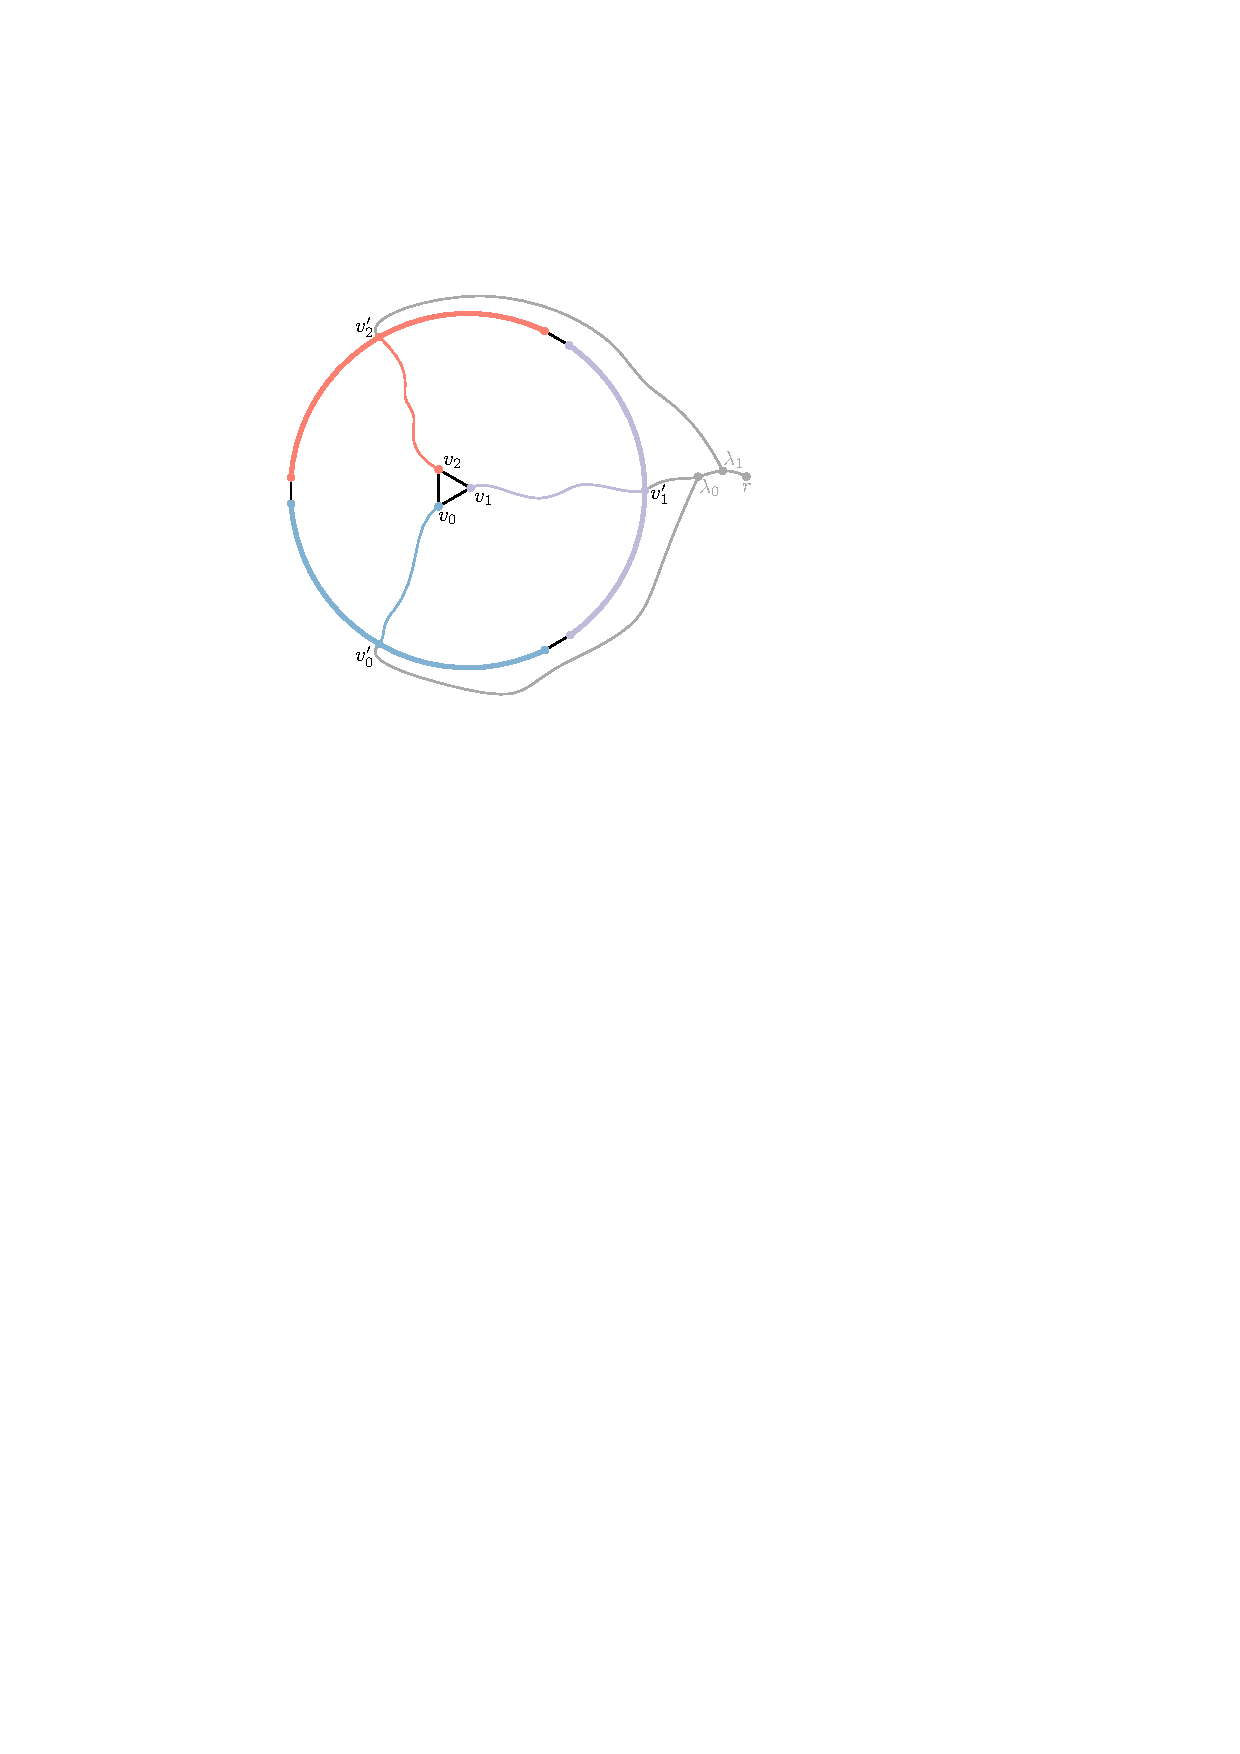
\includegraphics[page=1]{figs/second_case} &
      \includegraphics[page=2]{figs/second_case} \\
      (a) & (b) \\
      \includegraphics[page=3]{figs/second_case} &
      \includegraphics[page=4]{figs/second_case} \\
      (c) & (d) \\
    \end{tabular}
    \caption{The proof of \cref{three_w_csqrtn_quack}}
    \label{second_case_fig}
  \end{figure}

  The remainder of this proof is illustrated in \cref{second_case_fig}. Let $F_i$ be a face of $G_{i-1}$ that contains at least one vertex of $G$ in its interior.  Since $L_0\subseteq V(G_{i-1})$ contains the vertices on the outer face of $G$, $F_i$ is an inner face of $G_{i-1}$.  By (struct-a), $F_i$ is a cycle in $G$.  We first deal with the (hardest) case, in which $|I(F_i)|=3$ and then deal with the (degenerate) cases $|I(F_i)|\in\{1,2\}$.  Treat $F_i$ as a cycle.  By (struct-a) and (struct-b), the vertices of $F_i$ can be partitioned among three vertex-disjoint paths $P_0$, $P_1$, and $P_2$, each of which is contained in (the cycle) $F_i$ and such that, for each $\ell\in[3]$,  $V(P_\ell)\subseteq B_{j_\ell}$ for some $j_\ell\in[i]$.

  Let $G_{F_i}$ be the subgraph of $G$ induced by all vertices of $G$ in $F_i$ and all vertices of $G$ in the interior of the region bounded by $F_i$.  Since $F_i$ is an inner face of $G_{i-1}$, $G[L_0]$ is the outer face of $G$ and $r$ is in the outer face of $G$, each vertex $v\in V(G_F)$ has a $T$-ancestor in $V(F)$.  For each $v\in V(G_F)$ let $v'$ be the $T$-ancestor of $v$ in $V(F)$ that has maximum depth.  If $v'\in V(P_\ell)$, then define the \defin{colour} of $v$ to be $\ell$.  In this way, each vertex of $G_{F_i}$ is a assigned a colour from the set $[3]$.  Property (struct-b) and Sperner's Lemma imply that $G_{F_i}$ contains an inner face $\tau_i:=v_0v_1v_2$ for which the colour of $v_\ell$ is $\ell$, for each $\ell\in[3]$.  For each $\ell\in[3]$, let $Q_\ell:=\pth_T(v_\ell,v_\ell')$ be the path in $T$ from $v_\ell$ to the vertex $v_{\ell}'\in V(P_{\ell})$ whose colour determines that of $v_\ell$.

  The construction in \citet{dujmovic.joret.ea:planar} would, at this point, set $B_i:=\bigcup_{\ell=0}^2 V(Q_\ell-v_\ell')$.
  % (This is what \citet{dujmovic.joret.ea:planar} call a \defin{tripod}.)
  It is straightforward to verify that this choice of $B_i$ satisfies (good-a), (struct-a), and (struct-b).  By the choice of $\tau_i$ and $Q_0,Q_1,Q_2$, each face $F'$ of $G_i$ that is not a face of $G_{i-1}$ is contained in $F_i$ and avoids at least one of $P_0$, $P_1$, or $P_2$. Therefore, $F'$ avoids at least one of $B_{j_0}$, $B_{j_1}$ or $B_{j_2}$. Therefore $I(F')\subseteq \{j_0,j_1,j_2,i\}$ and does not contain at least one of $j_0$, $j_1$, or $j_2$, so $|I(F')|\le 3$, which ensures that $B_i$ satisfies (good-c) with $t=3$.  For any $j\in\N$, $|B_i\cap L_j|=\bigcup_{\ell=0}^2|V(Q_\ell)\cap L_j|\le 3$, so $B_i$ satisfies (good-b) with $w=3$.

  However, setting $B_i:=\bigcup_{\ell=0}^2 V(Q_\ell-v_\ell')$ could violate (good-c) and (struct-c), since there is no non-trivial upper bound on the length of the paths $Q_0$, $Q_1$, or $Q_2$.  We now explain the modifications needed to fix this.  First, observe that each of $Q_0$, $Q_1$, and $Q_2$ begins at a vertex of $\tau_i$.  Since $\tau_i$ is a clique, its vertices have $T$-depth\todo{Define $T$-depth} in $\{d,d+1\}$ for some integer $d$. If each of $Q_0$, $Q_1$, and $Q_2$ contains no more than $2\beta\sqrt{n}$ vertices, then $\spn(\mathcal{L},\bigcup_{\ell=0}^2 V(Q_\ell-v_\ell'))\le 2\beta\sqrt{n}$, so it satisfies (good-c) and (struct-c). In this case, we set $B_i:=\bigcup_{\ell=0}^2 V(Q_\ell-v_\ell')$ as before.

  Otherwise, assume without loss of generality that $|V(Q_1)|=\max\{|V(Q_\ell)|:\ell\in[3]\}\ge 2\beta\sqrt{n}$.  Since $v_1'\in V(P_1)$, (struct-c) implies that $\depth_T(v)\le \depth_T(v_1')+2\beta\sqrt{n}-1$ for each $v\in V(P_1)$.
  % Since there is an edge of $G$ from $P_0$ to $P_1$ and an edge of $G$ from $P_0$ to $P_2$, (struct-c) therefore implies that $\depth_T(v)\le \depth_T(v_1')+4\beta\sqrt{n}-2$ for each $v\in V(F)$. In particular, $\depth_T(v_1'),\depth_T(v_2')\le \depth_T(v_0')+4\beta\sqrt{n}-2$.

  % For each $\ell\in\{1,2,3\}$, $Q_\ell$ contains a vertex of depth $d\ge \depth_T(v_1')+c\sqrt{n}\ge \depth_T(v_1')+2(c/2)\sqrt{n}+1$, provided that $(c/2)\sqrt{n}+1\le c\sqrt{n}$, which is satisfied for all $c\ge\sqrt{3}$ and $n\ge 3$.  Therefore, for each $\ell\in\{1,2,3\}$, $Q_\ell$ contains a vertex $v_\ell''$ with $\depth_T(v_\ell'')=\depth_T(v_1')-1-\lceil (c/2)\sqrt{n}\rceil$.


  For each $\ell\in[3]$, Let $Q_\ell'$ be obtained from $Q_\ell$ by removing all vertices of depth greater than $\depth_T(v_1')+2\beta\sqrt{n}$.
  % Our set $B_i$ will contain $V(Q_1')$. Of course, this is not enough, since $Q_0'$, $Q_1'$, and $Q_2'$ may not separate the interior of $F_i$ in a way that maintains (good-c) [or (struct-a)--(struct-c) for that matter].
  % From this point on all subscripts on $Q$, $Q'$, $P$, and $v$ are implicitly taken modulo $3$.
  For each $\ell\in[2]$, let $\lambda_\ell$ be the lowest-common $T$-ancestor of $v_\ell$ and $v_{\ell+1}$.
  Let $C_\ell$ be the cycle formed by the edge $v_\ell v_{\ell+1}$,  $\pth_T(v_\ell,\lambda_\ell)$ and $\pth_T(v_{\ell+1}\lambda_\ell)$\todo{Define this notation}.

  For each $z\in\{1,2\}$ and $\ell\in[2]$, let $v_{\ell,z}$ be the $T$-ancestor of $v_\ell$ of $T$-depth $\depth_T(v_0)+\lceil z\beta\sqrt{n}\rceil$.  Note that $v_{\ell,z}$ is well-defined since $\depth_T(v_\ell)\ge d \ge \depth_T(v_0)+2\beta\sqrt{n}$.
  By \cref{awesome_path}, there exists a path $R_{\ell,z}$ from $v_{\ell,z}$ to $v_{\ell+1,z}$ in  $G_{C_\ell}$\todo{Define this notation} whose vertices have depths in the interval
  \begin{equation}
    \depth_T(v_{\ell,z}),\depth_T(v_{\ell,z})+\beta\sqrt{n}-1]
    \subseteq[\depth_T(v_0)+\lceil z\beta\sqrt{n}\rceil,\depth_T(v_0)+ (z+1)\beta\sqrt{n}] \label{face_span}
  \end{equation}
  and that contains at most $\alpha$ vertices from each layer in $\mathcal{L}$.

  Observe that $S_{z} := R_{0,z}\cup R_{1,z}$ is a path in $G$ with endpoints $v_{0,z}$ and $v_{2,z}$ that contains $v_{1,z}$ in its interior.  Let $X_{z}$ be the vertex set of the component of $S_{z}-V(F)$ that contains $v_{1,z}$.
  We set
  \[
     B_i := X_{1} \cup X_{2} \cup \bigcup_{\ell=0}^2 Q'_\ell\setminus V(F_i)
  \]
  All that remains is to verify that this choice of $B_i$ satisfies (good-a)--(good-c), (good-x), (good-s) and (struct-a)--(struct-c).
  \begin{description}
    \item[(good-a)] $B_i$ satisfies (good-a) since, by construction, all the vertices of $B_i$ are contained in the interior of $F_i$.

    \item[(good-b)] $B_i$ satisfies (good-b) for $w=2\alpha+3$ since, for any layer $L_j$, there is a $z\in\{1,2\}$ such that $|B_i\cap L_j|\le |L_j\cap (R_{0,z}\cup R_{1,z}\cup V(Q_0)\cup V(Q_1)\cup V(Q_2))|\le \alpha+\alpha+1+1+1$.  (The value $z=1$ if $j < \depth_T(v_1')+2\beta\sqrt{n}$ and $z=2$ otherwise.)

    \item[(good-x)] $B_i$ satisfies (good-x) for the following reasons: For any vertex $v$ in $S_1\cup S_2\cup Q_1'$, there is a path from $v_{1,2}$ to $v$.  For each $\ell\in\{1,2\}$, if $Q_\ell'$ is non-empty then $G[B_i]$ contains a path, namely $R_{\ell-1,2}$, from $v_{1,2}$ to the vertices in $Q'_\ell$.

    \item[(good-c)] This choice of $B_i$ satisfies (good-c) because $S_{2}$ cannot contain any vertices of $P_1$. Indeed, \cref{awesome_path} ensures that the vertices in $S_2$ have $T$-depth at least $\depth_T(v_1')+ 2\beta\sqrt{n}$ while (struct-c) ensures that the vertices in $P_1$ have $T$-depth at most $\depth_T(v_1')+2\beta\sqrt{n}-1$.

    Therefore $G_i$ contains a path $Q_0''$ whose internal vertices are contained $Q_0'\cup R_{0,2}$ from $v_{1,2}$ to some vertex in $P_0$.  $G'$ also has a path $Q_1''$ whose internal vertices are contained in $Q_1'$ from $v_{1,2}$ to some vertex in $P_1$.  $G'$ also has a path $Q_2''$ whose internal vertices are contained in $Q_2'\cup R_{1,2}$.  Consider the subgraph $G_i':=F\cup Q_0''\cup Q_1''\cup Q_2''$ of $G_i$

    Each inner face of $G_i'$ is incident to at most two of the paths $P_0$, $P_1$ or $P_2$ and is therefore incident to at most two of the vertex sets $B_{j_0}$, $B_{j_1}$ or $B_{j_2}$. Any face $F'$ of $G_i$ that is not a face of $G_{i-1}$ is contained in one of the inner faces of $G_i'$ and is therefore incident to at most three of $B_{j_0}$, $B_{j_1}$, $B_{j_2}$, or $B_i$.

    \item[(good-s)] $B_i$ satisfies (good-s) since all vertices in $B_i$ have depth at least $\depth_T(v_1')+1$ and (by \cref{face_span}) at most $\depth_T(v_1')+3\beta\sqrt{n}$.

    \item[(struct-a)] $B_i$ satisfies (struct-a) by construction.  In particular, $G_i$ can be obtained from $G_{i-1}$ by repeated adding a path between two vertices of a face whose inner vertices (this in $B_i=V(G_i)\setminus V(G_{i-1})$) are contained in the interior face.  The addition of each such path preserves biconnectivity.

    \item[(struct-b)] $B_i$ satisfies (struct-b) since $B_i$ is contained in the interior of a single face $F_i$ of $G_{i-1}$ and $G[B_i]$ is connected.  If $F'[B_i]$ were disconnected for some face $F'$ of $G_i$, then $G[B_i]$ would be disconnected.

    \item[(struct-c)] $B_i$ satisfies (struct-c) by \cref{face_span}.  Specifically, for any face $F'$ of $G_i$, the vertices in $B_i\cap V(F')$ come from vertices of $Q_1\cup Q_2\cup Q_3$ whose $T$-depths are in $[\depth_T(v_1')+(z-1)\beta\sqrt{n}+1,\depth_T(v_1')+z\beta\sqrt{n}]$, from vertices of $R_{0,z}$ and $R_{1,z}$ whose vertices $T$-depths are in $[\depth_T(v_1')+z\beta\sqrt{n},\depth_T(v_1')+(z+1)\beta\sqrt{n}]$, and (if $z=2$) vertices of $R_{0,z-1}$ and $R_{1,z-1}$ whose vertices $T$-depths are in $[\depth_T(v_1')+(z-1)\beta\sqrt{n},\depth_T(v_1')+z\beta\sqrt{n}]$. \qedhere
  \end{description}
\end{proof}



\section{Proof of \cref{awesome_path}}
\label{crux_section}

In this section, we prove \cref{awesome_path}.  Our approach is to show that $G_C$ contains a grid-like subgraph $G_C'$ where each layer of the grid contains vertices from the corresponding layer in the $\lambda$-rooted BFS layering of $G_C$. The vertices $s$ and $t$ are the leftmost and rightmost vertices in the top layer of $G_C'$.  Once we find this structure, finding the path from $s$ to $t$ is easy.  We take the zig-zag path that begins at $v_0:=s$ (in the leftmost column) and walk along the diagonal of the grid until reaching the rightmost column, then we take the vertical path in the rightmost column to reach $t$. The first part of this path, $v_0,w_0,v_1,w_1,\ldots,v_i,w_i$ uses at most two vertices, $v_j$ and $w_j$ in layer $j$ for each $j\in\{0,\ldots,i\}$ and uses at most two vertices, $w_j$ and $v_{j+1}$, in column $j+1$, for each $j\in\{0,\ldots,i-1\}$.

The second part of the path uses at most $1$ vertex in each of these layers, so the path uses at most $3$ vertices in each of the layers $0,\ldots,i$. To obtain a bound of $O(\sqrt{n})$ on the number, $i$, of layers, we will argue that $v_j$ is above at least $i-j$ vertices in its column.  Since $v_0,\ldots,v_i$ are all in different columns this implies that $G'_C$ contains at least $\sum_{j=0}^i(i-j+1)>i^2/2$ vertices.  Thus $i^2/2 < n$, so $i< \sqrt{2n}$.

Let $G$ be a connected planar graph and let $r$ be a vertex of $G$. To help us find the grid-like structure in $G_C$ we make use of the following concept from graph drawing. An \defin{ordered concentric representation} of $G$ with center $r$ is a non-crossing drawing of $G$ with $r$ on the outer face that has following properties:
\begin{compactenum}[(i)]
  \item For each $i\in\N$, the vertices in $L_i:=\{v\in V(G):\dist_G(v,r)=i\}$ are drawn on the line $y=-i$.
  \item For each edge $vw$ of $G$ with $v,w\in L_i$ for some $i$, the edge $vw$ is drawn as a curve whose interior is contained in the halfplane $y<-i$.
  \item For each edge $vw$ of $G$ with $v\in L_i$, $w\in L_{i+1}$ for some $i$, the edge $vw$ is drawn as the union of a curve $C_{vw}$ whose interior is contained in the strip $-i< y<i(i+1)$ and a curve $C_{wv}$ whose (possibly empty) interior is contained in the halfplane $y<-i(i+1)$.
\end{compactenum}

\citet{pupyrev:mixed} proves that every connected planar graph has a such a representation:

\begin{lem}\label{pupyrev}
  For every connected planar graph $G$ and every vertex $r$ of $G$, there exists an ordered concentric representation of $G$ with center $r$.
\end{lem}

From this point on, we fix a vertex $r$ of our triangulation $G$ and an ordered concentric representation of $G$ centered at $r$.  We do not distinguish between a vertex and the point that represents it or between an edge and the curve that represents it.  We use the words ``left'' and ``right'' to compare two vertices on the same layer in the natural way.  We use ``above'' and ``below'' to compare layers or to compare a vertex to a layer.

We say that an edge $vw$ of $G$ is a \defin{clean} edge if, for some $i$, $v\in L_i$, $w\in L_{i+1}$ and the interior of $vw$ is entirely contained in the strip $-i < y -(i-1)$.  The vertices $v$ and $w$ are called the \defin{upper} and \defin{lower} endpoints of $vw$.  The following strengthening of \cref{pupyrev} will allow us to build a spanning tree consisting entirely of clean edges.  Ultimately, vertical paths in this spanning tree will be used to construct columns in the grid-like graph $G_C'$.

\begin{lem}\label{clean_edge}
  For every triangulation $G$ and every vertex $r$ of $G$, there exists an ordered concentric representation of $G$ with center $r$ such that, for each vertex $w\neq r$, the vertex $w$ is the lower endpoint of at least one clean edge.
\end{lem}

\begin{proof}
  First, suppose that $w\in L_{i+1}$ is not on the outer face of $G$.  Then one of the faces $F:=uvw$ of $G$ incident to $w$ contains a non-empty line segment $wx$, where $x$ is a point above layer $i+1$. At least one of $u$ or $v$ must be in $L_{i}$ since, otherwise, the interior of $uvw$ is completely below layer $i+1$. Without loss of generality, assume $v\in L_i$. Let $F'$ be the intersection of the interior of $F$ with the halfplane $y<-(i+1)$. Then $F'$ is connected and contains $w$ and $v$ on its boundary.  If the edge $vw$ is not clean, then it can be redrawn in the interior of $F'$ so that it is clean.

  When $w$ is a vertex of the outer face, the argument is almost the same, except that the face incident to $w$ that contains the line segment $wx$ may be the outer face.  In this case, we chose $v\in L_i$ such that $vw$ is an edge of the outer face. If it is not already clean, then the edge $vw$ can be redrawn so that it is clean.
\end{proof}

Let $T$ be the subgraph of $G$ obtained by choosing, for each vertex $w\in V(G)\setminus\{r\}$, a clean edge whose lower endpoint is $w$.  Clearly $T$ is acyclic, and it has $n-1$ edges, so $T$ must contain the vertex $r$, so $T$ is a spanning tree of $G$ that consists entirely of clean edges.  We treat $T$ as a rooted tree whose root is $r$.  Then, for each $i\in\N$ and each $v\in L_i$, $\depth_T(v)=i$.

% For a node $v\in L_i$, the $T$-children $v_0,\ldots,v_{k-1}\in L_{i+1}$ have a natural left-to-right order given by their order in $L_{i+1}$.  This gives a natural left-to-right order for the subtrees $T_0,\ldots,T_{k-1}$ of $T$ rooted at these nodes.  Define the relationship $\prec$ over pairs of vertices $v,w$ of $G$ as follows:  If neither of $v$ or $w$ is a $T$-ancestor of the other, then the $x$ be the lowest common $T$-ancestor of $v$ and $w$, let $v'$ be the second node in $\pth_T(x,v)$ and let $w'$ be the second node in $\pth_T(x,w)$.  Then $v\prec w$ if $v'$ is to the left of $w'$, and $w\prec v$ if $w'$ is to the left of $v'$.

Consider the following relation $\prec$ over pairs of vertices in $G$. For each $i$ and each pair of distinct vertices $v,w\in L_i$, $v\prec w$ if and only if  $v$ is to the left of $w$.  For a pair of vertices $v\in L_i$ and $w\in L_j$, with $j>i$, let $w'$ be the $T$-ancestor of $w$ whose $T$-depth is $i$.  If $v\prec w'$ then $v\prec w$. If $w'\prec v$ then $w\prec v$. (If $v=w'$ then $v$ and $w$ are incomparable.)

% \begin{clm}
%   There is no sequence of vertices $v_0,\ldots,v_{k-1}$ in $G$ such that $v_0\prec_0 v_1\prec_0\cdots\prec_0 v_{k-1}\prec_0 v_0$.
% \end{clm}
%
% \begin{proof}
%   Let $i$ be the minimum integer such that $\{v_0,\ldots,v_{k-1}\}\subseteq \bigcup_{j>i}L_i$.  For each $j\in[k]$, let $v'_j$ be the $T$-ancestor of $v_j$ in $L_i$.  If $v_0',\ldots,v_{k-1}'$ are all distinct, then $v_0'$ is the leftmost of these vertices in $L_i$ and $v_{k-1}'$ is the rightmost of these vertices in layer $i$.
% \end{proof}
%
%
% Let $\prec$ be the transitive closure of $\prec_0$.

\begin{obs}
  For any two vertices $v,w\in V(G)$, exactly one of the following is true:
  \begin{compactenum}
    \item $v$ is a $T$-ancestor of $w$ or $w$ is a $T$-ancestor of $v$; or
    \item $v\prec w$ or $w\prec v$.
  \end{compactenum}
\end{obs}

% \begin{clm}\label{partial_order}
%   The pair $(V(G),\prec)$ is a strict partial order.
% \end{clm}
%
% \begin{proof}
%   We need to show that $\prec$ is irreflexive, asymmetric, and transitive.  By definition $v\not\prec v$ for any $v\in V(G)$, so $\prec$ is irreflexive.
%
%   If $v\prec w$ for $v,w\in L_i$ then $v\not\prec w$ because the ``left of'' relationship is a total order. Next, consider the case that $v\prec w$ for $v\in L_i$ and $w\in L_j$, $i\neq j$.  In this case, $v\prec w$ if and only if $v'\prec w'$, where $v'$ and $w'$ are the $T$-ancestors of $v$ and $w$ in $L_{\min\{i,j\}}$.  Again, this implies that $w'\not\prec v'$, which implies that $w\not\prec v$.  Thus, $\prec$ is asymmetric.
%
%   If $u\prec v$ and $v\prec w$ then.....
% \end{proof}


% \begin{clm}
%   For each edge $vw\in E(G)\setminus E(T)$, $v\prec w$ or $w\prec v$.
% \end{clm}
%
% \begin{proof}
%   If $v,w\in L_i$ for some $i$ then this is immediate. Otherwise $v\in L_i$ and $w\in L_{i+1}$ for some $i$. Let $w'$ be the parent of $w$ in $T$.  Then $w'\in L_i$ and, since $vw\not\in E(T)$, $w'\neq v$.  Therefore $w'$ is comparable to $v$, so $w$ is comparable to $v$.
% \end{proof}


We say that a vertex $z\in L_j$ is \defin{$i$-redundant} if there exists an edge $vw\in E(G)\setminus E(T)$ such that $v\prec z\prec w$ and $v\in L_{i'}$ for some $i'\le i$.

\begin{clm}\label{has_descendant}
  If $i\ge j$, and a vertex $v\in L_j$ is not $i$-redundant then $v$ has a $T$-descendant\todo{Define $T$-descendant} in $L_i$.
\end{clm}

\begin{proof}
  If $v$ is on the outer face of $G_C$, then the result is trivial since the two paths that define the outer face of $G_C$ are paths in $T$.\todo{This is where we assume that the BFS tree is special.}  Therefore, we may assume that $v$ is not on the outer face of $G_C$.

  The proof is by induction on $i-j$.
  If $i=j$, the result is trivial since $v$ is a $T$-descendant of itself. For $i>j$, it suffices to show that $v$ has at least one non-redundant $T$-child $v'$ after which we can apply induction on $v'\in L_{j+1}$.

  If $v$ has no child in $T$, then there is a face $vxy$ with $x\prec v\prec y$ and $x,y\in L_{j}\cup L_{j+1}$. Then $x$ and $y$ have $T$-ancestors $x'$ and $y'$ in $L_j$ (possibly $x=x'$ or $y=y'$). But this implies that $v$ is $(j+1)$-redundant, a contradiction. We now assume that $v$ has at least one child in $T$.

  Let $v_1\prec\cdots\prec v_k$ be the $T$-children of $v$.  Note that every vertex of $G_C$ on the line segment $\overline{v_1v_k}$ is a child of $v$.  Planarity implies that if $v_1,\ldots,v_k$ are all $i$-redundant then there is a single edge $xy$ with endpoints in $L_{j+1}\cup\cdots\cup L_i$ such that $x$ has a $T$-ancestor $x'\in L_{j+1}$ with $x'\prec v_1$ and $y$ has a $T$-ancestor $y'\in L_{j+1}$ with $v_k\prec y'$. Let $x''$ be the parent of $x'$ and let $y''$ be the parent of $y'$.  Neither $x'$ nor $y'$ is a child of $v$, so $x''\neq v$ and $y''\neq v$. The edges $x'x''$ does not cross the edge $vv_1$, so $x''\prec v$.  Similarly, $v\prec y''$.  Therefore $x''\prec v\prec y''$, which implies that $v$ is $i$-redundant, a contradiction.
\end{proof}


Let $C$, $G_C$, $s$, $t$, and $d$ be defined as in \cref{awesome_path}, with the restriction that the tree $T$ in \cref{awesome_path} is the tree $T$ defined above.  In all of the following, we use the convention that $s\prec t$.  A path $P$ in $G_C$ is \defin{$(i,b)$-suitable} if $V(P)\subseteq L_{d}\cup\cdots L_{d+i}$ and $|V(P)\cap L_j|\le b$ for all $j\in\N$.  A vertex $v\in V(G_C)$ is \defin{$(i,b)$-reachable} if $G_C$ contains an $(i,b)$-suitable path from $s$ to $v$.

\todo[inline]{There's an annoying mismatch here, where many occurrences of $i$ and $j$ should be replaced with $i+d$ and $j+d$ since we want everything to be relative to $d=\depth_T(s)=\depth_T(t)$.}


% \begin{clm}
%   If $v,w\in L_j\cap V(G_C)$, such that $w$ is $(i,b)$-reachable, $v\prec w$, and $v$ is not $i$-redundant then $v$ is $(i,b)$-reachable.
% \end{clm}
%
% \begin{proof}
%   Since $w$ is $(i,b)$-reachable, $j\le i$.
%   If $s$ is a $T$-ancestor of $v$ then this is trivial, since $\pth_T(s,v)$ is an $(i,b)$-suitable path from $s$ to $v$.  Otherwise, $s\prec v$.
%   Let $P$ be an $(i,b)$-suitable path from $s$ to $w$.  We claim that $P$ contains a vertex $v'$ that is incomparable to $v$.  Since $v\prec w$, the only other possibility is that $P$ contains an edge $v'w'$ with $v'\prec v$ and $v\prec w'$. If $v'w'$ is above $v$ then $v'w'$ crosses an edge of $\pth(r,v)$, which is not possible since $G$ is a non-crossing drawing.  If $v'w'$ is below $v$ then $v$ is redundant, which is not possible by the assumptions of the lemma.
%
%   Thus $P$ contains a vertex $v'$ that is incomparable to $v$. The path $P$ therefore consists of two subpaths $P_{sv'}$ and $P_{v'w}$ with a common endpoint $v'$.  Note that the path $P_{v'w}$ contains at least one vertex from each layer between the layer that contains $v'$ and the layer that contains $w$.  The path $\pth(v',v)$ intersects each of these layers in exactly one vertex.  Therefore, the concatenation of $P_{sv'}$ and $\pth(v',v)$ is an $(i,b)$-suitable path from $s$ to $v$.
% \end{proof}

\begin{clm}
   Let $G_C'$ be the subgraph of $G_C$ obtained by removing every $i$-redundant vertex of $G_C$.  Let $v_1\prec\cdots\prec v_r$ be be the vertices in $L_j\cap V(G_C')$.  Then $G_C'$ contains the path $v_1,\ldots,v_r$.
\end{clm}

\begin{proof}
  Consider the vertex $v_p$ for some $p\in\{1,\ldots,r-1\}$. Some face $uv_pw$ of $G_C$ contains a horizontal line segment of positive length whose left endpoint is $v_p$.  At least one of the vertices of this face, say $w$, is in $L_j$. Therefore $G_C$ contains at least one edge $v_pv'$ with $v_p\prec v'$ and $v'\in L_j$.  Let $v'$ be such an edge that maximizes $v'$, with respect to $\prec$.  The existence of the edge $v_pv'$ implies that all vertices of $G_C$ in the interior of the segment $v_pv'$ are $j$-redundant and therefore $i$-redundant.  Furthermore, planarity implies that if $v'$ is $i$-redundant, then so is $v_p$, which contradicts the fact that $v_p$ is a vertex of $G_C'$.  Therefore $v'=v_{p+1}$ and $G_C'$ contains the edge $v_pv_{p+1}$ as required.  This is true for all $p\in\{1,\ldots,r-1\}$, so $v_1,\ldots,v_p$ is a path in $G_C'$.
\end{proof}


\begin{clm}
   Let $G_C'$ be the subgraph of $G_C$ obtained by removing every $i$-redundant vertex of $G_C$.  Let $v_1\prec\cdots\prec v_r$ be be the vertices in $L_j\cap V(G_C')$.  Then $G_C'$ contains the path $v_1,\ldots,v_r$.
\end{clm}

\begin{proof}
  Consider the vertex $v_p$ for some $p\in\{1,\ldots,r-1\}$. Some face $uv_pw$ of $G_C$ contains a horizontal line segment of positive length whose left endpoint is $v_p$.  At least one of the vertices of this triangle, say $w$ is in $L_j$. Therefore $G_C$ contains at least one edge $v_pv'$ with $v_p\prec v'$ and $v'\in L_j$.  Let $v'$ be such an edge that maximizes $v'$, with respect to $\prec$.  The existence of the edge $v_pv'$ implies that all vertices of $G_C$ in the interior of the segment $v_pv'$ are $j$-redundant and therefore $i$-redundant.  Furthermore, planarity implies that if $v'$ is $i$-redundant, then so is $v_p$, which contradicts the fact that $v_p$ is a vertex of $G_C'$.  Therefore $v'=v_{p+1}$ and $G_C'$ contains the edge $v_pv_{p+1}$ as required.  This is true for all $p\in\{1,\ldots,r-1\}$, so $v_1,\ldots,v_p$ is a path in $G_C'$.
\end{proof}


\begin{clm}\label{bam}
  Let $G_C'$ be the subgraph of $G_C$ obtained by removing every $i$-redundant vertex of $G_C$.  Then $t$ is $(i,3)$-reachable or $|V(G_C')|\ge i^2/2$.
\end{clm}

\begin{proof}
  Starting from $v_0:=s\in L_d$, construct a path as follows:  Suppose that after $j$ iterations, we have constructed a path from $s$ to a vertex $v_j\in L_{d+j}$ that contains at most two vertices from each of $L_d,\ldots,L_{d+j-1}$ and contains only the vertex $v_j\in L_j$.  If $v_j$ has neighbour $w_j\in L_{d+j}$ with $v_j\prec w_j$ then add $w_j$ to the path.  Then add any $T$-child $v_{j+1}$ of $w_j$.  If $v_j$ has no such neighbour, then $v_j$ is a $T$-descendant of $t$ and we complete the path to $t$ with $\pth_T(v_j,t)$.

  If this process completes in at most $i$ iterations then the resulting path is $(i,3)$-suitable.  Otherwise, by \cref{has_descendant}, the vertex $v_j$ has a $T$-descendant in each of $L_{j+1},\ldots,L_i$. It follows immediately from the definitions that $v_0\prec\cdots\prec v_i$, so none of these vertices is a $T$-ancestor of any other.  Therefore, the total number $T$-descendants of $v_0,\ldots,v_i$ is at least
  \[
    \sum_{j=0}^i (i-j+1) = \sum_{j=1}^{i+1} j = (i+1)(i+2)/2 > i^2/2 \enspace .
    \qedhere
  \]
\end{proof}

\begin{proof}[Proof of \cref{awesome_path}]
  Since $G_C$ has at most $n$ vertices, \cref{bam}, with $i=\lceil \sqrt{2n}\rceil$ implies that $G_C$ contains a path that satisfies the conditions of the lemma.
\end{proof}

\section{Products with Paths}

\section{Bounded Genus Graphs}


\bibliographystyle{plainurlnat}
\bibliography{short_tripods}


\end{document}
